\documentclass{beamer}
%\documentclass[handout]{beamer}
% This file is a solution template for:

% - Giving a talk on some subject.
% - The talk is between 15min and 45min long.
% - Style is ornate.

% Copyright 2004 by Till Tantau <tantau@users.sourceforge.net>.
%
% In principle, this file can be redistributed and/or modified under
% the terms of the GNU Public License, version 2.
%
% However, this file is supposed to be a template to be modified
% for your own needs. For this reason, if you use this file as a
% template and not specifically distribute it as part of a another
% package/program, I grant the extra permission to freely copy and
% modify this file as you see fit and even to delete this copyright
% notice. 


\mode<presentation>
{
  \usetheme{Montpellier}

  %\setbeamercovered{transparent}
  % or whatever (possibly just delete it)
}

\usepackage{xmpmulti} % package that defines \multiinclude

\usepackage[english]{babel}

\usepackage[latin1]{inputenc}

\usepackage{times}
\usepackage[T1]{fontenc}
% Or whatever. Note that the encoding and the font should match. If T1
% does not look nice, try deleting the line with the fontenc.

%\title [short title] (optional, use only with long paper titles)
\title{The Context Algorithm}

\author[Freund] % (optional, use only with lots of authors)
{Yoav Freund}
% - Give the names in the same order as the appear in the paper.
% - Use the \inst{?} command only if the authors have different
%   affiliation.

\institute[Universities of Somewhere and Elsewhere] % (optional, but mostly needed)

\subject{Machine Learning}
% This is only inserted into the PDF information catalog. Can be left
% out. 

% If you have a file called "university-logo-filename.xxx", where xxx
% is a graphic format that can be processed by latex or pdflatex,
% resp., then you can add a logo as follows:

% \pgfdeclareimage[height=0.5cm]{university-logo}{university-logo-filename}
% \logo{\pgfuseimage{university-logo}}



% Delete this, if you do not want the table of contents to pop up at
% the beginning of each subsection:
%% \AtBeginSubsection[]
%% {
%%   \begin{frame}<beamer>
%%     \frametitle{Outline}
%%     \tableofcontents[currentsection,currentsubsection]
%%   \end{frame}
%% }


% If you wish to uncover everything in a step-wise fashion, uncomment
% the following command: 

\beamerdefaultoverlayspecification{<+->}

\newcommand{\newmcommand}[2]{\newcommand{#1}{{\ifmmode {#2}\else\mbox{${#2}$}\fi}}}
\newcommand{\renewmcommand}[2]{\renewcommand{#1}{{\ifmmode {#2}\else\mbox{${#2}$}\fi}}}
\newcommand{\newmcommandi}[2]{\newcommand{#1}[1]{{\ifmmode {#2}\else\mbox{${#2}$}\fi}}}
\newcommand{\newmcommandii}[2]{\newcommand{#1}[2]{{\ifmmode {#2}\else\mbox{${#2}$}\fi}}}
\newcommand{\newmcommandiii}[2]{\newcommand{#1}[3]{{\ifmmode {#2}\else\mbox{${#2}$}\fi}}}

\newcommand{\algfnt}{\bf}

\newmcommand{\ouralg}{{\mbox{\algfnt Hedge}({\eta})}}

\newmcommand{\iter}{T}

\newfont{\cmmib}{cmmib10}
\newcommand{\boldell}{{\mbox{\cmmib \symbol{'140}}}}


\newmcommandi{\costvec}{{\boldell}_{#1}}
\newmcommandii{\cost}{{\ell}^{#1}_{#2}}

\newmcommandi{\rd}{\tilde{#1}}

\newmcommandi{\distvec}{{\bf p}^{#1}}
\newmcommandi{\rddistvec}{\rd{\bf p}^{#1}}
\newmcommandii{\dist}{{p}^{#1}_{#2}}
\newmcommandii{\rddist}{\rd{p}^{#1}_{#2}}

\newmcommandi{\bdistvec}{{\bf q}^{#1}}
\newmcommandii{\bdist}{{q}^{#1}_{#2}}

\newmcommandi{\wtvec}{{\bf w}^{#1}}
\newmcommandi{\rdwtvec}{\rd{\bf w}^{#1}}
\newmcommandii{\wt}{{w}^{#1}_{#2}}
\newmcommandii{\rdwt}{\rd{w}^{#1}_{#2}}


\newcommand{\Nweight}[2]{V_{#1}^{#2}}	%the normalized weight
\newcommand{\dweight}[2]{w^{#2}(#1)} % initial density measure
\newcommand{\TEloss}[1]{L_{#1}}	%total loss of expert i
\newcommand{\BEloss}{L_{\min}}	%total loss of the best expert
\newcommand{\TAloss}{L_A}	%total loss of algorithm
\newcommand{\weight}[2]{W_{#1}^{#2}} % weight assigned to expert
\newcommand{\btheta}{\hat{\theta}}

\newcommand{\R}[1]{{\color{red}{#1}}}
\newcommand{\B}[1]{{\color{blue}{#1}}}
\newcommand{\RM}[1]{{\color{red}{$#1$}}}


%BANDITS
\newcommand{\Aplay}{{\bf Hedge}}
\newcommand{\Aest}{{\bf Exp3}}
\newcommand{\Aesthp}{{\bf Exp3.P}}
\newcommand{\Aestg}{{\bf Exp3.P.1}}
\newcommand{\Aests}{{\bf Exp3.S}}
\newcommand{\Aessg}{{\bf Exp3.S.1}}
\newcommand{\Astrat}{{\bf Exp4}}
\newcommand{\Abound}{{\bf Exp3.1}}
\newcommand{\Gbest}{G_{\rm max}}

\newcommand{\defeq}{\stackrel{\rm def}{=}}
\newcommand{\compl}{\mbox{\sc h}}
\newcommand{\theset}[2]{\{ {#1} \,:\, {#2} \}}

\newmcommandii{\stratv}{\mbox{\boldmath $\xi$}^{#1}({#2})}

%Games paper
\newmcommand{\M}{\bf M}
\newmcommand{\dM}{\M'}
\newmcommand{\Row}{\bf R}
\newmcommand{\dRow}{\R'}
\newmcommand{\C}{\bf C}
\newmcommand{\dC}{\C'}
\newmcommand{\D}{D}
\renewmcommand{\P}{\bf P}
\newmcommand{\Q}{\bf Q}
\newmcommand{\Dt}{\D_t}
\newmcommand{\Pt}{\P_t}
\newmcommand{\Qt}{\Q_t}
\newmcommand{\Pstar}{\P^*}	% the min/max optimal mixed strategy
\newmcommand{\Pref}{\tilde{\P}}	% a reference mixed strategy (not
				% necessarily min/max)
\newmcommand{\Qstar}{\Q^*}
\newmcommand{\Pa}{\overline{\P}}
\newmcommand{\Qa}{\overline{\Q}}
\newmcommand{\Qh}{\hat{\Q}}
\newmcommandi{\trans}{{#1}^{\rm T}}
\newmcommand{\mhx}{\M(h,x)}
\newmcommand{\mxh}{\dM(x,h)}
\newmcommand{\mpq}{\M(\P,\Q)}
\newmcommand{\mpsq}{\M(\Pstar,\Q)}
\newmcommand{\mpsqt}{\M(\Pstar,\Qt)}
\newmcommand{\mptqt}{\M(\Pt,\Qt)}
\newmcommand{\mptt}{\M(\Pt,t)}
\newmcommand{\mptq}{\M(\Pt,\Q)}
\newmcommand{\mpqt}{\M(\P,\Qt)}
\newcommand{\minp}{\min_{\P}}
\newcommand{\maxq}{\max_{\Q}}
\newcommand{\RE}[2]{{\rm RE}\left( {#1} \; \parallel \; {#2} \right) }

\newmcommand{\sumt}{\sum_{t=1}^T}
\newmcommand{\sumin}{\sum_{i=1}^n}
\newmcommand{\delt}{\Delta_{T,n}}
\newcommand{\nextline}{\vspace{0.2cm}\\}   % a little space for equation arrays

\newcommand{\lwalg}{\mbox{\rm MW}}
\newcommand{\lwalgvar}{\mbox{\rm vMW}}

%%
\newcommand{\E}{\mbox{\rm\bf E}}
\newcommand{\p}[2]{p_{#1}(#2)}
\newcommand{\q}[2]{q_{#1}(#2)}
\newcommand{\x}[2]{x_{#1}({#2})}
\newmcommand{\bx}{\mbox{\boldmath$x$}}
\newmcommandi{\xv}{\bx({#1})}
\newmcommand{\xvt}{\xv{t}}
%\newcommand{\w}[2]{w_{#1}({#2})} replaced by \wt, but remember to switch order of parameters i and t
\renewcommand{\i}[1]{i_{#1}}
\newcommand{\hx}[2]{\hat{x}_{#1}(#2)}
\newcommand{\hxit}{\hx{\i{t}}{t}}
\newcommand{\pit}{\p{\i{t}}{t}}
\newcommand{\xit}{\x{\i{t}}{t}}
\newcommand{\expb}[1]{\exp\left(#1\right)}

\newcommand{\vp}{{\mathbf p}}
\newcommand{\vu}{{\mathbf u}}
\newcommand{\vv}{{\mathbf v}}
\newcommand{\vx}{{\mathbf x}}
\newcommand{\vy}{{\mathbf y}}
\newcommand{\vw}{{\mathbf w}}
\newcommand{\vq}{{\mathbf q}}

\newcommand{\vecq}{{\bf q}}
\newcommand{\vecp}{{\bf p}}


\newcommand{\HedgeLoss}{L_{\mbox{\footnotesize Hedge}}}

\newcommand{\W}{\vec{W}}
\newcommand{\V}{\vec{V}}
\newcommand{\X}{\vec{X}}
\newcommand{\vb}{\vec{b}}
%\newcommand{\loss}{\vec{\ell}}
\newcommand{\loss}{L}
\newcommand{\elloss}[2]{\ell_{#2}\left( #1 \right)} %loss of expert i at time t
\newcommand{\lossvec}[1]{{\mathbf \ell}_{#1}}       %loss of expert at time t
\newcommand{\w}[1]{\makebox[12pt]{{#1}}}
\newcommand{\Rps}{\mbox{\tt R}}
\newcommand{\rPs}{\mbox{\tt P}}
\newcommand{\rpS}{\mbox{\tt S}}
\newcommand{\rpstie}{\w{$\frac{1}{2}$}}
\newcommand{\rpswin}{\w{$0$}}
\newcommand{\rpsloss}{\w{$1$}}

\newmcommand{\decspace}{\Delta}
\newmcommand{\decsym}{\delta}
\newmcommandi{\dec}{\decsym^{#1}}
\newmcommand{\decdistsym}{\cal D}
\newmcommandi{\decdist}{{\decdistsym}^{#1}}

\newmcommand{\simpdistspace}{{\bf \cal S}}
\newmcommand{\domset}{{\rm dom}(\decdistsym)}

\newmcommand{\expdistsym}{{\cal E}}
\newmcommandii{\expdist}{{\expdistsym}^{#1}_{#2}}
\newmcommand{\expdecsym}{{\varepsilon}}
\newmcommandii{\expdec}{\expdecsym^{#1}_{#2}}

\newmcommand{\outspace}{\Omega}
\newmcommand{\outsym}{\omega}
\newmcommandi{\out}{\outsym^{#1}}

%\newmcommandii{\Dkl}{D_{\mbox{kl}}\paren{#1||#2}}
\newmcommandii{\Dkl}{{\rm {KL}}\paren{{#1}\;||\;{#2}}}

\newmcommandi{\sumwts}{\sum_{i=1}^N \wt{#1}{i}}

\newmcommand{\lossalg}{L_A}
\newmcommand{\lossouralg}{{L_{\mbox{\scriptsize\algfnt Hedge}(\eta)}}}
\newmcommand{\lossS}{{L_{\mbox{\scriptsize\algfnt S}}}}
\newmcommandi{\lossi}{L_{#1}}
\newmcommandii{\lossit}{L_{#1}^{#2}}

\newmcommandi{\upbnd}{\tilde{#1}}

\newcommand{\angles}[1]{{\left\langle {#1} \right\rangle}}
\newcommand{\paren}[1]{{\left( {#1} \right)}}
\newcommand{\brac}[1]{{\left[ {#1} \right]}}
\newcommand{\braces}[1]{{\left\{ {#1} \right\}}}

\newcommand{\abs}[1]{{\left| {#1} \right|}}
\newcommand{\ceiling}[1]{{\left\lceil {#1} \right\rceil}}

\newfont{\msym}{msbm10}
\newcommand{\real}{\mbox{\msym R}}

\newmcommand{\updatefcn}{U_\eta}

%% \newtheorem{theorem}{Theorem}	
%% \newtheorem{lemma}[theorem]{Lemma}
%% \newtheorem{corollary}[theorem]{Corollary}
%% \newtheorem{definition}{Definition}

%\newcommand{\proof}{\noindent{\bf Proof:} }
%\newcommand{\example}[1]{{\em Example #1.} }
%\newcommand{\qed}{\rule{0.7em}{0.7em}}

\newcommand{\WeakAlg}{\mbox{\algfnt WeakLearn}}
\newcommand{\Boost}{\mbox{\algfnt AdaBoost}}
\newcommand{\EX}{\mbox{\bf EX}}
\newmcommand{\hf}{h_{{f}}}
\newmcommand{\rdhf}{\rd{h}_{{f}}}
\newmcommand{\hfT}{h^T_{{f}}}
\newmcommand{\ranh}{{b}}

\newmcommand{\conclass}{{\cal C}}

\newmcommand{\badvec}{{\bf b}}
\newmcommandi{\bad}{{b}_{#1}}

%%%%%%%% New commands defined for the game-playing paper

\newmcommand{\hedge}{\algfnt Hedge}
\newmcommand{\play}{\algfnt Play}
\newmcommandi{\Glossvec}{{\bg y}^{#1}}
\newmcommandii{\Gloss}{{y}^{#1}_{#2}}
%\newmcommandi{\action}{{I}_{#1}}
\newmcommandi{\Gdistvec}{{\bf \tilde{p}}^{#1}}
\newmcommandii{\Gdist}{{\teilde{p}}^{#1}_{#2}}

%%%%%%%%%%%%%%%%%%%%%%%%%%%%%%%%%%%%%%%%%%%%%%%%%%%%%
\newmcommand{\Idistvec}{{D}}
\newmcommandi{\Idist}{\Idistvec({#1})}
\newmcommand{\Idistt}{\Idistvec_t}

\newmcommand{\Xdist}{{\cal P}}
\newmcommand{\emp}{\hat{\epsilon}}

\newmcommand{\classpc}{Y}
\newmcommand{\numclass}{k}
\newmcommandii{\prob}{\mbox{\rm Pr}_{#1}\left[{#2}\right]}
\newmcommandii{\exval}{\mbox{\rm E}_{#1}\left[{#2}\right]}

%\usepackage{amsmath}
\DeclareMathOperator*{\argmax}{argmax} % thin space, limits underneath in displays
\DeclareMathOperator*{\argmin}{argmin} 

\newcommand{\RR}{\mathbb{R}}
\newcommand{\regret}{\mbox{Regret}}

%%% Conditional probabilities
\newmcommandii{\condp}{p\left( #1 \left| #2 \right. \right)}

\newmcommand{\lab}{y}
\newmcommand{\ploss}{\mbox{ploss}}
\newmcommandii{\avploss}{\ploss_{#1}({#2})}
\newcommand{\sfrac}[2]{\mbox{$\frac{#1}{#2}$}}

\newcommand{\mboosta}{\mbox{\algfnt AdaBoost.M1}}
\newcommand{\mboostb}{\mbox{\algfnt AdaBoost.M2}}
\newcommand{\mboostr}{\mbox{\algfnt AdaBoost.R}}

%\newmcommand{\slos}{\mbox{ploss}}
%\newmcommandiii{\sloss}{\slos_{#1}({#2},{#3})}
%\newmcommandiii{\avsloss}{\slos_{{#1},{#2}}({#3})}

\newmcommandii{\vwt}{{W}^{#1}_{#2}}

\newcommand{\figline}{\rule{\textwidth}{1pt}}

%\newmcommandi{\1}{{\bf 1}({#1})}
\newmcommandi{\1}{[\![{#1}]\!]}

\newmcommand{\confcn}{\kappa}
\newmcommandi{\erint}{\abs{\int_{y_i}^{h_t(x_i)} {#1} dy}}
%\newmcommandi{\erint}{\int_{\min\{y_i,h_t(x_i)\}}^{\max\{y_i,h_t(x_i)\}}{#1}dy}


\begin{document}

%\iffalse %%%%%%%%%%%%%%%%%%%%%%%%%%%%%%%%%%%%%%%%%%%%%%%%%%%%%%%%%%%%%%%%%%

\begin{frame}
  \titlepage
\end{frame}

\begin{frame}
  \frametitle{Outline}
  \tableofcontents[pausesections]
  % You might wish to add the option [pausesections]
\end{frame}

\section{Review}

\begin{frame}
\frametitle{The online Bayes Algorithm}
\begin{itemize}
\item {\color{blue} Total loss} of expert \R{$i$}
\R{$$L_i^t = - \sum_{s=1}^{t} \log p_i^s(c^s);\;\;\; L_i^0 = 0$$}
\item {\color{blue}Weight} of expert \R{$i$}
\R{$$\wt{t}{i} = \wt{1}{i} e^{-L_i^{t-1}} = \wt{1}{i} \prod_{s=1}^{t-1} p_i^s(c^s)$$}
\item
Freedom to choose initial weights.\\
 \R{$\wt{1}{t} \geq 0$}, \R{$\sum_{i=1}^n \wt{1}{i} = 1$}
\item {\color{blue}Prediction} of algorithm \R{$A$}
\R{\[
\vp_A^t = \frac{\sum_{i=1}^N \wt{t}{i} \vp_i^t}{\sum_{i=1}^N \wt{t}{i}}
\]}
\end{itemize}
\end{frame}

\begin{frame}
\frametitle{Cumulative loss vs. Final total weight}

\onslide<1-> Total weight: \R{$W^t \doteq \sum_{i=1}^N \wt{t}{i}$}

\onslide<2-> \R{$$
\frac{W^{t+1}}{W^t}  =  \frac{\sum_{i=1}^N \wt{t}{i} e^{\log p_i^t(c^t)}}{\sum_{i=1}^N \wt{t}{i}} 
\onslide<3->          =   \frac{\sum_{i=1}^N \wt{t}{i} p_i^t(c^t)}{\sum_{i=1}^N \wt{t}{i}} 
\onslide<4->        =  p_A^t(c^t)
$$}
\onslide<5-> \R{$$ -\log \frac{W^{t+1}}{W^t} = -\log p_A^t(c^t) $$}
\R{\[
\onslide<8-> -\log W^{T+1} =
\onslide<6-> -\log \frac{W^{T+1}}{W^1} = -\sum_{t=1}^T \log p_A^t(c^t)
\onslide<7-> = L_A^T
\]}
\onslide<9-> \R{\bf EQUALITY} not bound!
\end{frame}

\begin{frame}
\frametitle{Simple Bound}
\begin{itemize}
\item Use non-uniform initial weights \R{$\sum_i \wt{1}{i} = 1$}
\item Total Weight is at least the weight of the best expert.
\R{\begin{eqnarray*}
L_A^T & = & -\log W^{T+1} 
\pause = -\log \sum_{i=1}^N \wt{T+1}{i} \\
\pause & = & -\log \sum_{i=1}^N \wt{1}{i} e^{-L_i^T} 
\pause \leq  - \log \max_i \paren{ \wt{1}{i} e^{-L_i^T} } \\
\pause & = & \min_i \paren{ L_i^T -\log \wt{1}{i} }
\end{eqnarray*}}
\end{itemize}
\end{frame}

\begin{frame}
\frametitle{Universal Online coding}
  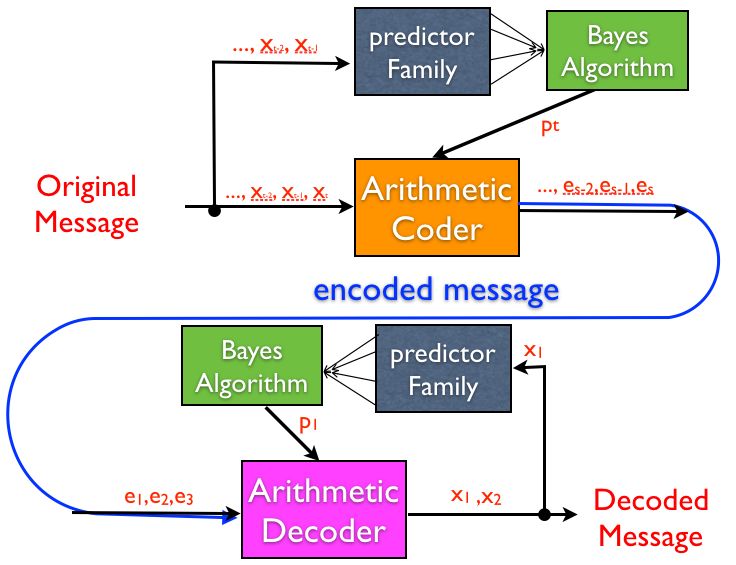
\includegraphics[width=3in]{figures/ArithmeticCoding_key.png}
\end{frame}

\begin{frame}
\frametitle{Combining large predictor families}
  \begin{itemize}
\item
  Log loss is {\bf mixable} = each predictor in the family can use a
  Bayesian combination of a family of sub-predictors, with no
  additional loss.
\item We talked about the KT preictor.
\item Today we consider the much richer set of variable length
  markov models.
\item The set of predictors is of exponential size, but the
  algorithm is efficient.
\end{itemize}
\end{frame}

\section{Fixed Length Markov Models}

%An Example
\begin{frame}
\frametitle{A fixed length Markov Model}
\begin{columns}
\begin{column}[t]{8cm}
\begin{itemize}
\item Observe a binary sequence.
\item \R{$x_1,\ldots,x_{t-1}$}
\item Predict next bit from past
\item \R{$P(x_t=1 | x_{t-1},x_{t-2},\ldots,x_1)$}
\item Use only last \R{$k$} bits
\item \R{$P(x_t=1 | x_{t-1},\ldots,x_{t-k})$}
\item Markov model of order \R{$k$}
\end{itemize}
\end{column}
\begin{column}[T]{5cm}
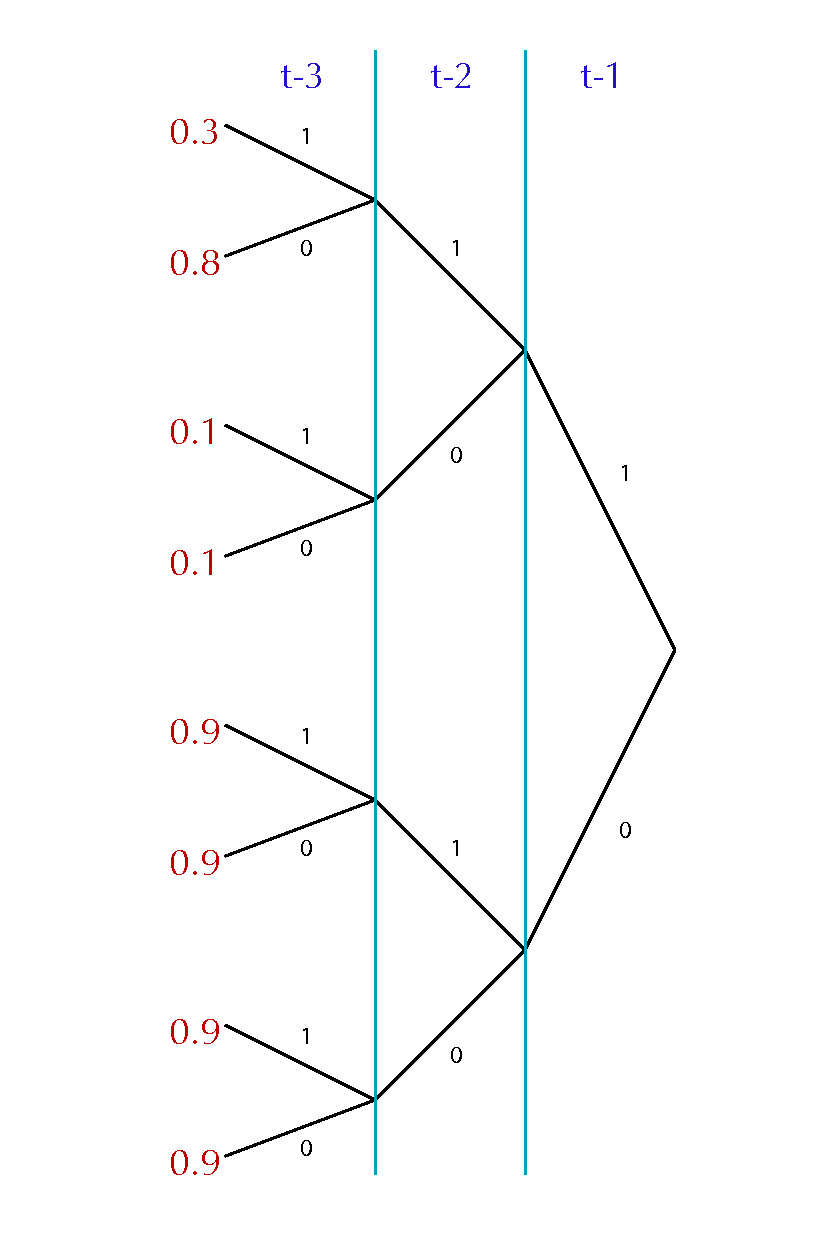
\includegraphics[width=4.5cm]{figures/PredictionTree.pdf}
\end{column}
\end{columns}
\end{frame}

%Using the KT predictor in each element
\begin{frame}
\frametitle{Learning a markov distribution}
\begin{itemize}
\item Each tree leaf is associated with a binary sequence
\R{$y_1,\ldots,y_k$} 
\item For each leaf keep two counters:
\begin{itemize}
\item \R{$a_{y_1,\ldots,y_k}$} = number of times \R{$x_{t-1}=y_1, \ldots, x_{t-k}=y_k$} \\ and \R{$x_t=0$}
\item \R{$b_{y_1,\ldots,y_k}$} = number of times \R{$x_{t-1}=y_1, \ldots, x_{t-k}=y_k$} \\ and \R{$x_t=1$}
\end{itemize}
\item Prediction (using Kritchevski Trofimov)
\R{\[p(x_t=1 | x_{t-1}=y_1,\ldots,x_{t-k}=y_k) 
= \frac{b_{y_1,\ldots,y_k}+1/2}{a_{y_1,\ldots,y_k}+b_{y_1,\ldots,y_k}+1}\]}
\item Total regret is at most \R{$2^{k-1} \log T$}
\end{itemize}
\end{frame}

\section{Variable Length Markov Model (VMM)}

%Why variable length is better than fixed length. (QU example)

\begin{frame}
\frametitle{How variable length markov can reduce regret}
\begin{columns}
\begin{column}[T]{5cm}
\multiinclude[graphics={width=4.5cm},format=pdf]{figures/PredictionTree}
\end{column}
\begin{column}[t]{8cm}
\begin{itemize}
\item Reducing number of leaves from \R{$8$} to \R{$4$} means 
\item reducing regret from \R{$4 \log T$} to \R{$2 \log T$}
\item English example: \\
\B{B \pause A \pause R \pause O \pause Q }\pause \R{U} \pause \B{E}
\item When we have little data, we can get better prediction even if the children are not 
\B{Exactly the same}
\end{itemize}
\end{column}
\end{columns}
\end{frame}

%defining complete trees
\begin{frame}
\frametitle{Prefix trees / Tries}
\begin{itemize}
\item In a prefix binary tree each node has either \R{0} or \R{2} children.
%\item A node with \R{1} child means that some past histories are not
%  covered.
\item A variable length markov model corresponds to a \B{prefix tree}.
\item You can think of a prefix trees as different \B{prunings} of a
  maximal tree.
\item We don't know a-priori which pruning to use!
\item The number of prunings trees increases exponentially with the
  number of nodes in the maximal tree.
\item We will use the Online Bayes to predict almost as well as the
  best prefix tree in hind-sight.
\item First - simple but inefficient algorithm, Second - efficient algorithms.
\end{itemize}
\end{frame}

% \section{Assigning weights to trees}

% Using bayesian method to perform almost as well as the best VMM
\section{Universal coding, an inefficient solution}

\begin{frame}
\frametitle{Using online Bayes to learn the structure}
\begin{itemize}
\item We assign to each tree an initial weight of \R{$2^{-n}$} where
  \R{$n$} is the number of \B{nodes} in the  pruned tree.
\item We combine the predictions of the trees using online Bayes.
\item The total regret would be \R{$\frac{l}{2}\log T + n$} where \R{$l$} is the number of \B{leaves} in the prefix tree.
%\item The papers do things slightly differently because they bound the depth of the tree by \R{$k$}.
\item This algorithm maintains a weight for each prefix tree.
\item The number of prunings of a full tree of depth $k$ is
  $O(2^{2^k})$ while maintaining all of the counts requires $O(2^k)$. 
\end{itemize}
\end{frame}

% Defining the distribution using a random process.

\section{Efficient Implementation}

\iffalse
\begin{frame}
\frametitle{Efficient implementation}
\begin{itemize}
\item \B{First idea:} Estimate probabilities of complete sequences and use conditional to generate predictions.
\item The prior weights are used for averaging the complete sequence probabilities - they don't need to be updated.
\item \B{Second idea:} Compute the average over the prior efficiently.
\end{itemize}
\end{frame}
\fi


\begin{frame}
\frametitle{Efficient generation of prior}
\begin{itemize}
\item Prior distribution is generated by a stochastic recursion.
\item Start with root node (always exists)
\item For each node flip a fair coin.
\begin{itemize}
\item \B{Heads} Set node to be a leaf (\R{0} children)
\item \B{Tails} Create \R{2} children nodes to the node.
\end{itemize}
\item Defines a distribution over all prefix trees.
\item Probability of a tree with \R{$n$} nodes is \R{$2^{-n}$}
\end{itemize}
\end{frame}

% computing the posterior takes linear time because we can use the
% random process definition.
\begin{frame}
\frametitle{Efficient averaging over the prior (observations)}
\begin{itemize}
\item Maintain a KT estimator at each node of the tree.
\item Allocate counters only for nodes that have been visited.
\item At iteration \R{$t$} only \R{$t$} counters need to be updated.
\item Only \R{$k$} counters if depth of tree is bounded.
\item Each node is visited on a subset of the iterations.
\item Subset corresponding to node is contained in subset corresponding to node's parent.
\end{itemize}
\end{frame}

\begin{frame}
\frametitle{Efficient averaging over the prior (procedure)}
\begin{itemize}
\item This is not the method used in the original paper, it appears in
  a later paper by \em{Willems, Tjalkens and Ignatenko}. Available on
  github.
\end{itemize}
\end{frame}

\begin{frame}
\frametitle{Definitions}
\begin{itemize}
\item \R{$s$} is a bit sequence corresponding to a node in the
  tree. The chidren of this node are \R{$0s$} and \R{$1s$}.
\item The sequence of past bits up to time \R{$t$} is denoted
  \R{$x_1^{t-1}$}, the \R{$t$}'th bit is denoted \R{$X_t$}
\item \R{$s$} determines a subsequence of \R{$x_1^{t-1}$}: the locations
  preceded by the reverse of \R{$s$}.
\item \R{$a_s(x_{1}^{t-1}), b_s(x_{1}^{t-1})$} count the number of 0's
  and 1's in the subsequence corresponding to \R{$s$}
\item     The KT estimate associated with node \R{$s$}.
  \R{$$
    P_e^s\paren{X_t=1 | x_1^{t-1}} = \frac{b_s(x_1^{t-1})+1/2}{a_s(x_1^{t-1})+b_s(x_1^{t-1})+1}
          $$}
\end{itemize}
\end{frame}

\begin{frame}
\frametitle{Assigning probabilities to complete sequences}
\begin{itemize}
\item Using the chain rule, we can use a prediction rule to 
assign probabilities to a complete sequence.
\R{\[
P \paren{x_1=y_1,\ldots,x_T=y_T} = p \paren{x_1=y_1} p\paren{x_2=y_2|x_1=y_1} \ldots
\]}
\item
We can translate probabilities for complete sequences back into predictions.
\R{\begin{eqnarray*}
p \paren{ x_t=1 | x_1=y_1,\ldots,x_{t-1}=y_{t-1}} = \\
\frac{p\paren{x_1=y_1,\ldots,x_{t-1}=y_{t-1},x_t=1}}
{p\paren{x_1=y_1,\ldots,x_{t-1}=y_{t-1}}}
\end{eqnarray*}}
\end{itemize}
\end{frame}

\begin{frame}
\frametitle{Mixing Factors}
\begin{itemize}
\item \R{$P_w^s\paren{X_t=1 | x_1^{t-1}}$} The posterior average of
  the predictions associated with the descendants of the node \R{$s$}.
\item Using the chain rule we can also define unconditional
  probabilities \R{$P_w^s\paren{x_1^{t-1}}$}
\item The mixing factors according to the \B{Prior} distribution is
  0.5: stop, 0.5: continue
\item After observing \R{$x_1^{t-1}$} the odds change. The updated
  odds are represented by \R{$\beta^s(x_1^{t-1})$}:
\item \R{$P_w^s\paren{X_t=1 | x_1^{t-1}}$} The posterior average of
  the predictions associated with the descendants of the node \R{$s$}.
\end{itemize}
\end{frame}

\begin{frame}
\frametitle{Outline of algorithm}
\begin{itemize}
\item {\bf Forward}: Traverse the tree from root to leaf.
\item {\bf extend}: Add two children to the leaf. Initialized counts
  to 0,1.
\item {\bf Backward traversal}: Traverse back to root.\\
  For each node
  \R{$s$}
  \begin{itemize}
  \item compute \R{$P_e^s\paren{X_t=1 | x_1^{t-1}}$} and
      \R{$P_w^s\paren{X_t=1 | x_1^{t-1}}$}
    \item update counts: \R{$a^s,b^s$}.
    \item update \R{$\beta^s$}
    \end{itemize}
  \end{itemize}
\end{frame}

\section{Slides from Frans Willems}
\newpage
\bf{Slides from Frans Willems}\\
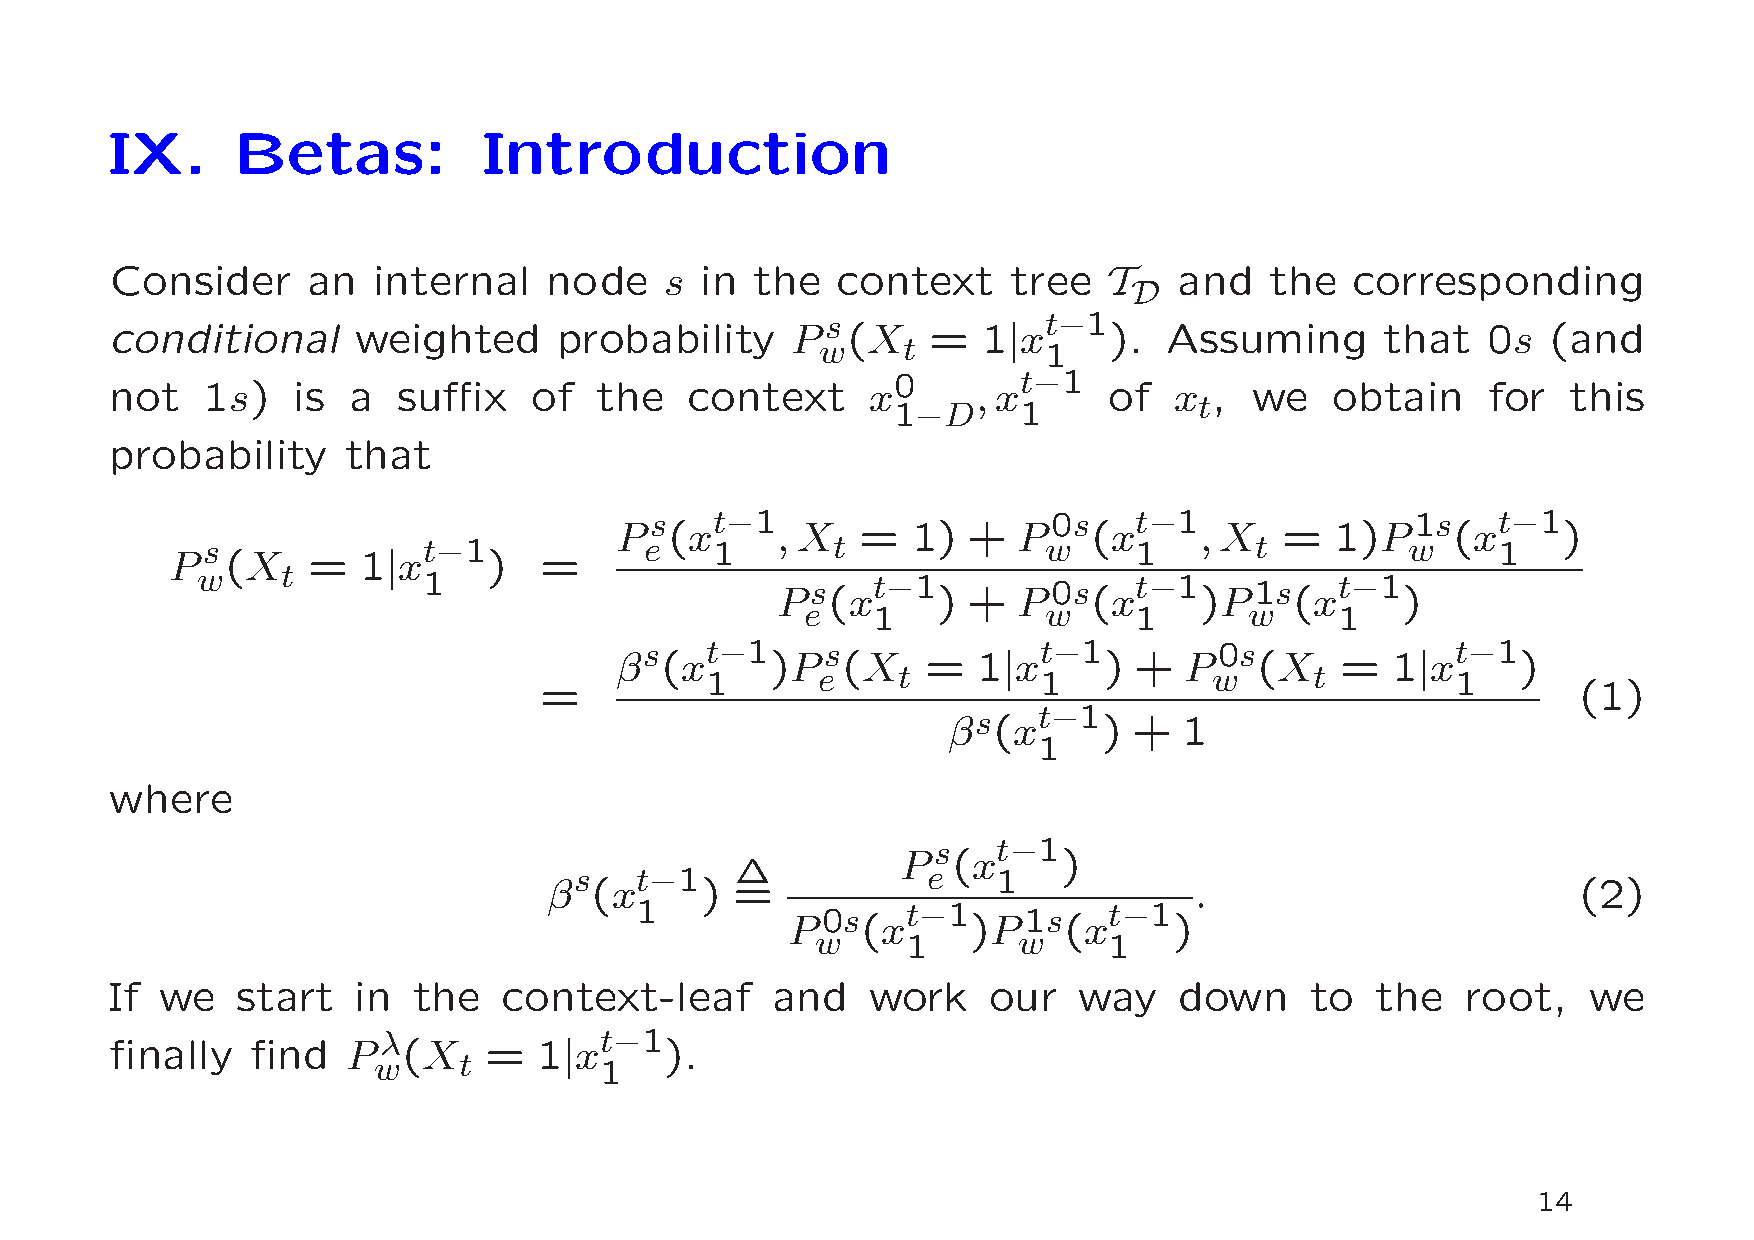
\includegraphics[width=4in]{figures/Betas1.pdf}

\newpage
\bf{Slides from Frans Willems}\\
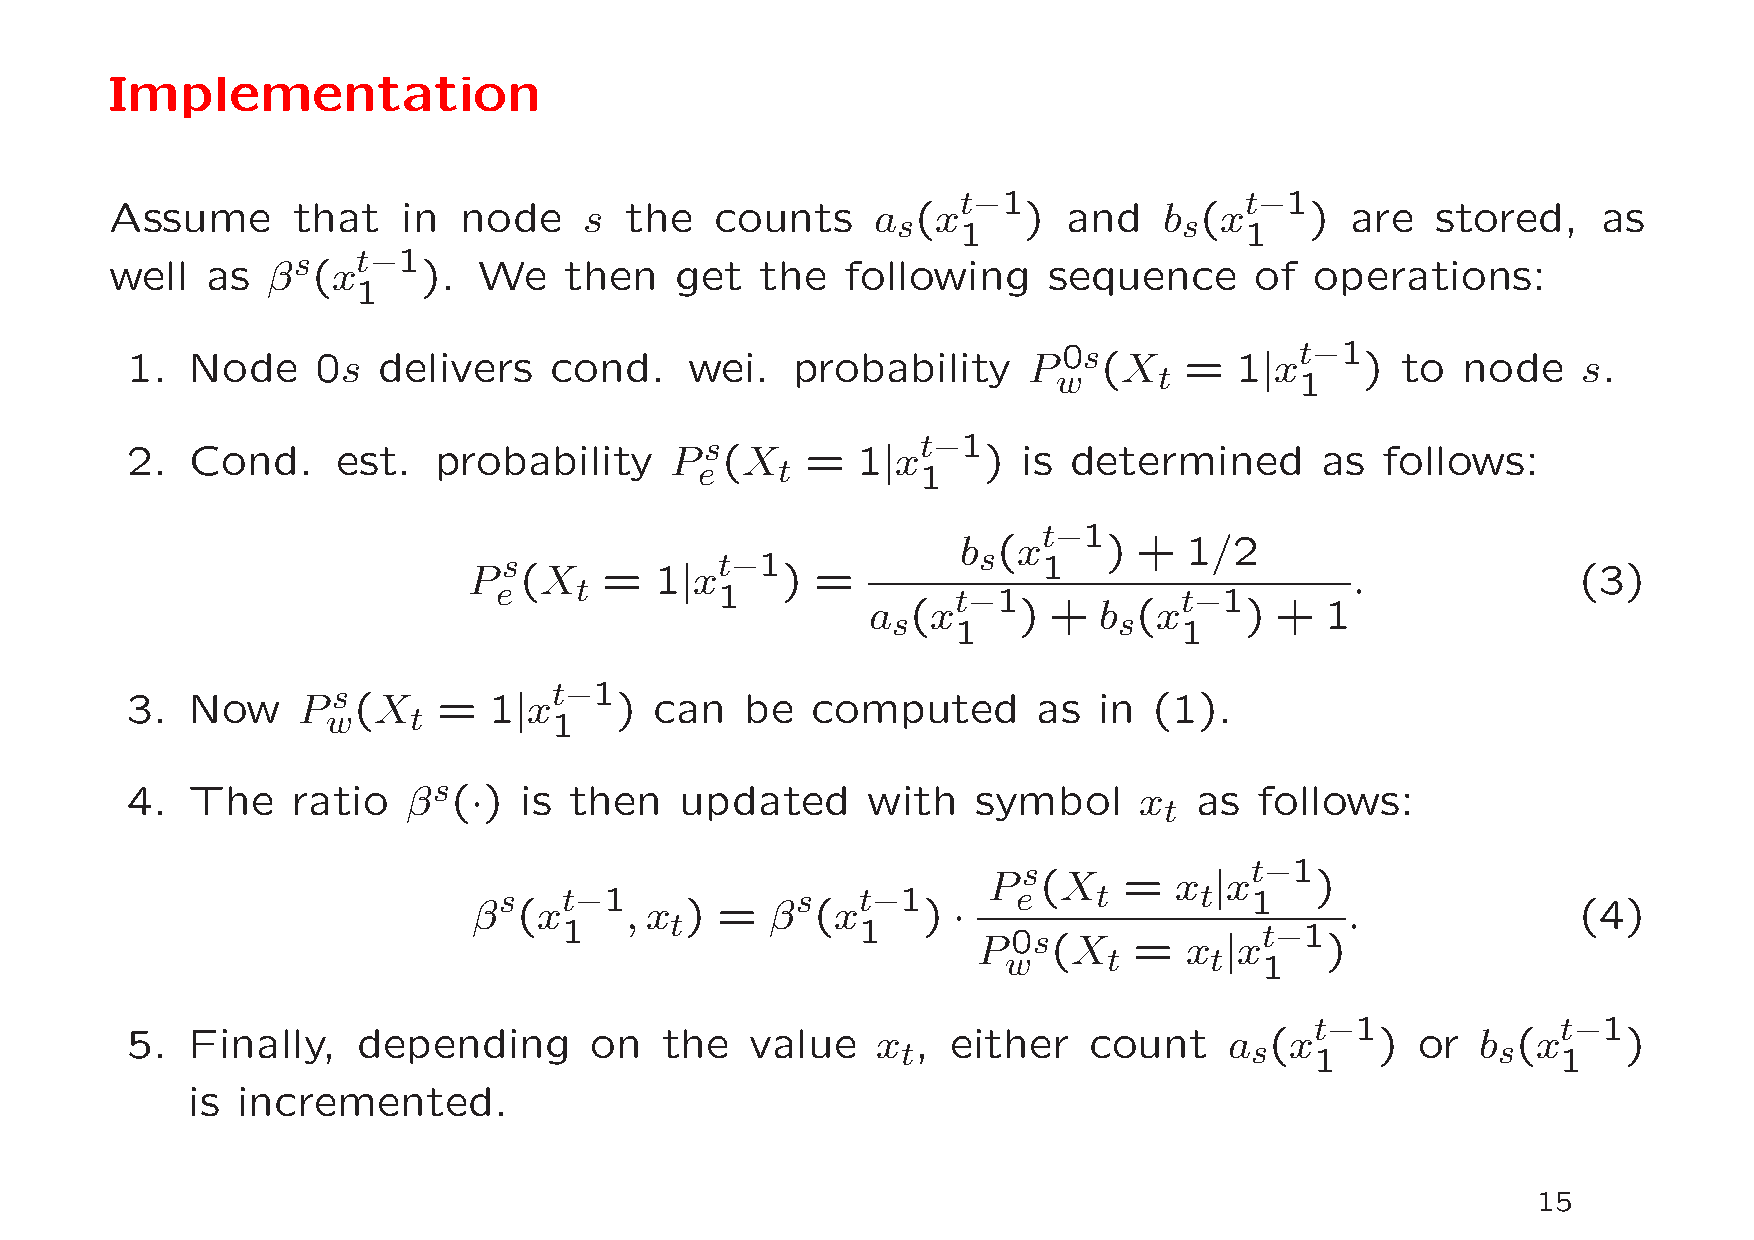
\includegraphics[width=4in]{figures/Betas2.pdf}

\begin{frame}
  \frametitle{Binary Tree}
  Sequence: 0,0,1,1,0,1,0,1,0,1,1,0,1,1,1\\~\\
  
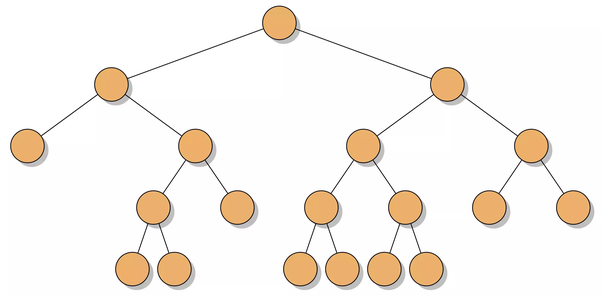
\includegraphics[width=4in]{figures/BinaryTree.png}
\end{frame}

% Recaping the algorithm.

% generalizing the algorithm to Hedge.

% Next class thursday.


\end{document}


